% vim: set textwidth=120:

% Example CV based on the 1.5-column-cv template. Main features:
% * uses the Roboto font family and IcoMoon icon set;
% * doesn't use colours, different font weights are used instead for styling;
% * because the CV fits on one page, header and footer is empty, since there isn't much useful info to put there;
% * includes a photo.
\documentclass[a4paper,10pt]{article}


% package imports
% ---------------

\usepackage[british]{babel} % for correct language and hyphenation and stuff
\usepackage{calc}           % for easier length calculations (infix notation)
\usepackage{enumitem}       % for configuring list environments
\usepackage{fancyhdr}       % for setting header and footer
\usepackage{fontspec}       % for fonts
\usepackage{geometry}       % for setting margins (\newgeometry)
\usepackage{graphicx}       % for pictures
\usepackage{microtype}      % for microtypography stuff
\usepackage{xcolor}         % for colours


% margin and column widths
% ------------------------

% margins
\newgeometry{left=15mm,right=15mm,top=15mm,bottom=15mm}

% width of the gap between left and right column
\newlength{\cvcolumngapwidth}
\setlength{\cvcolumngapwidth}{3.5mm}

% left column width
\newlength{\cvleftcolumnwidth}
\setlength{\cvleftcolumnwidth}{44.5mm}

% right column width
\newlength{\cvrightcolumnwidth}
\setlength{\cvrightcolumnwidth}{\textwidth-\cvleftcolumnwidth-\cvcolumngapwidth}

% set paragraph indentation to 0, because it screws up the whole layout otherwise
\setlength{\parindent}{0mm}


% style definitions
% -----------------
% style categories explanation:
% * \cvnameXXX is used for the name;
% * \cvsectionXXX is used for section names (left column, accompanied by a horizontal rule);
% * \cvtitleXXX is used for job/education titles (right column);
% * \cvdurationXXX is used for job/education durations (left column);
% * \cvheadingXXX is used for headings (left column);
% * \cvmainXXX (and \setmainfont) is used for main text;
% * \cvruleXXX is used for the horizontal rules denoting sections.

% font families
\defaultfontfeatures{Ligatures=TeX} % reportedly a good idea, see https://tex.stackexchange.com/a/37251

\newfontfamily{\cvnamefont}{Roboto Medium}
\newfontfamily{\cvsectionfont}{Roboto Medium}
\newfontfamily{\cvtitlefont}{Roboto Regular}
\newfontfamily{\cvdurationfont}{Roboto Light Italic}
\newfontfamily{\cvheadingfont}{Roboto Regular}
\setmainfont{Roboto Light}

% colours
\definecolor{cvnamecolor}{HTML}{000000}
\definecolor{cvsectioncolor}{HTML}{000000}
\definecolor{cvtitlecolor}{HTML}{000000}
\definecolor{cvdurationcolor}{HTML}{000000}
\definecolor{cvheadingcolor}{HTML}{000000}
\definecolor{cvmaincolor}{HTML}{000000}
\definecolor{cvrulecolor}{HTML}{000000}

\color{cvmaincolor}

% styles
\newcommand{\cvnamestyle}[1]{{\Large\cvnamefont\textcolor{cvnamecolor}{#1}}}
\newcommand{\cvsectionstyle}[1]{{\normalsize\cvsectionfont\textcolor{cvsectioncolor}{#1}}}
\newcommand{\cvtitlestyle}[1]{{\large\cvtitlefont\textcolor{cvtitlecolor}{#1}}}
\newcommand{\cvdurationstyle}[1]{{\small\cvdurationfont\textcolor{cvdurationcolor}{#1}}}
\newcommand{\cvheadingstyle}[1]{{\normalsize\cvheadingfont\textcolor{cvheadingcolor}{#1}}}


% inter-item spacing
% ------------------

% vertical space after personal info and standard CV items
\newlength{\cvafteritemskipamount}
\setlength{\cvafteritemskipamount}{5mm plus 1.25mm minus 1.25mm}

% vertical space after sections
\newlength{\cvaftersectionskipamount}
\setlength{\cvaftersectionskipamount}{2mm plus 0.5mm minus 0.5mm}

% extra vertical space to be used when a section starts with an item with a heading (e.g. in the skills section),
% so that the heading does not follow the section name too closely
\newlength{\cvbetweensectionandheadingextraskipamount}
\setlength{\cvbetweensectionandheadingextraskipamount}{1mm plus 0.25mm minus 0.25mm}


% intra-item spacing
% ------------------

% vertical space after name
\newlength{\cvafternameskipamount}
\setlength{\cvafternameskipamount}{3mm plus 0.75mm minus 0.75mm}

% vertical space after personal info lines
\newlength{\cvafterpersonalinfolineskipamount}
\setlength{\cvafterpersonalinfolineskipamount}{2mm plus 0.5mm minus 0.5mm}

% vertical space after titles
\newlength{\cvaftertitleskipamount}
\setlength{\cvaftertitleskipamount}{1mm plus 0.25mm minus 0.25mm}

% value to be used as parskip in right column of CV items and itemsep in lists (same for both, for consistency)
\newlength{\cvparskip}
\setlength{\cvparskip}{0.5mm plus 0.125mm minus 0.125mm}

% set global list configuration (use parskip as itemsep, and no separation otherwise)
\setlist{parsep=0mm,topsep=0mm,partopsep=0mm,itemsep=\cvparskip}


% CV commands
% -----------

% creates a "personal info" CV item with the given left and right column contents, with appropriate vertical space after
% @param #1 left column content (should be the CV photo)
% @param #2 right column content (should be the name and personal info)
\newcommand{\cvpersonalinfo}[2]{
    % left and right column
    \begin{minipage}[t]{\cvleftcolumnwidth}
        \vspace{0mm} % XXX hack to align to top, see https://tex.stackexchange.com/a/11632
        \raggedleft #1
    \end{minipage}% XXX necessary comment to avoid unwanted space
    \hspace{\cvcolumngapwidth}% XXX necessary comment to avoid unwanted space
    \begin{minipage}[t]{\cvrightcolumnwidth}
        \vspace{0mm} % XXX hack to align to top, see https://tex.stackexchange.com/a/11632
        #2
    \end{minipage}

    % space after
    \vspace{\cvafteritemskipamount}
}

% typesets a name, with appropriate vertical space after
% @param #1 name text
\newcommand{\cvname}[1]{
    % name
    \cvnamestyle{#1}

    % space after
    \vspace{\cvafternameskipamount}
}

% typesets a line of personal info beginning with an icon, with appropriate vertical space after
% @param #1 parameters for the \includegraphics command used to include the icon
% @param #2 icon filename
% @param #3 line text
\newcommand{\cvpersonalinfolinewithicon}[3]{
    % icon, vertically aligned with text (see https://tex.stackexchange.com/a/129463)
    \raisebox{.5\fontcharht\font`E-.5\height}{\includegraphics[#1]{#2}}
    % text
    #3

    % space after
    \vspace{\cvafterpersonalinfolineskipamount}
}

% creates a "section" CV item with the given left column content, a horizontal rule in the right column, and with
% appropriate vertical space after
% @param #1 left column content (should be the section name)
\newcommand{\cvsection}[1]{
    % left and right column
    \begin{minipage}[t]{\cvleftcolumnwidth}
        \raggedleft\cvsectionstyle{#1}
    \end{minipage}% XXX necessary comment to avoid unwanted space
    \hspace{\cvcolumngapwidth}% XXX necessary comment to avoid unwanted space
    \begin{minipage}[t]{\cvrightcolumnwidth}
        \textcolor{cvrulecolor}{\rule{\cvrightcolumnwidth}{0.3mm}}
    \end{minipage}

    % space after
    \vspace{\cvaftersectionskipamount}
}

% creates a standard, multi-purpose CV item with the given left and right column contents, parskip set to cvparskip
% in the right column, and with appropriate vertical space after
% @param #1 left column content
% @param #2 right column content
\newcommand{\cvitem}[2]{
    % left and right column
    \begin{minipage}[t]{\cvleftcolumnwidth}
        \raggedleft #1
    \end{minipage}% XXX necessary comment to avoid unwanted space
    \hspace{\cvcolumngapwidth}% XXX necessary comment to avoid unwanted space
    \begin{minipage}[t]{\cvrightcolumnwidth}
        \setlength{\parskip}{\cvparskip} #2
    \end{minipage}

    % space after
    \vspace{\cvafteritemskipamount}
}

% typesets a title, with appropriate vertical space after
% @param #1 title text
\newcommand{\cvtitle}[1]{
    % title
    \cvtitlestyle{#1}

    % space after
    \vspace{\cvaftertitleskipamount}
    % XXX need to subtract cvparskip here, because it is automatically inserted after the title "paragraph"
    \vspace{-\cvparskip}
}


% header and footer
% -----------------

% set empty header and footer
\pagestyle{empty}



% preamble end/document start
% ===========================

\begin{document}


% personal info
% -------------

\cvpersonalinfo{
    % photo
    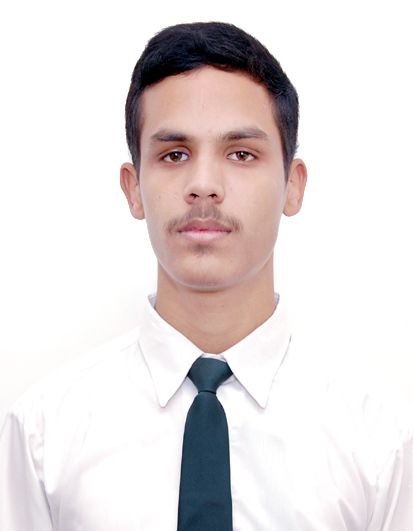
\includegraphics[height=36mm]{photo.jpg}
}{
    % name
    \cvname{SURYANSH SINGH RATHORE}

    % address
    \cvpersonalinfolinewithicon{height=4mm}{location_logo.png}{
        House No. C-1013, Indira Nagar, Near Church, Lucknow-226016
    }

    % phone number
    \cvpersonalinfolinewithicon{height=4mm}{call_logo.png}{
        +91 7990774698
    }

    % email address
    \cvpersonalinfolinewithicon{height=4mm}{gmail_logo.png}{
        rathoresuryansh196@gmail.com
    }

    % LinkedIn account
    \cvpersonalinfolinewithicon{height=4mm}{linkedin_logo.jpeg}{
        https://www.linkedin.com/in/suryansh-singh-rathore-9a1342159/
    }
    
    % Github account
    \cvpersonalinfolinewithicon{height=4mm}{git_logo.png}{
        https://github.com/rathoresuryansh196
    }
}

\cvsection{OBJECTIVE}

\vspace{\cvbetweensectionandheadingextraskipamount}
\cvitem{
    \cvdurationstyle{ }
}{
    %\cvtitle{ }

    To work in an environment which gives me handful opportunities to learn and explore new technologies around the world.

}
% education
% ---------

\cvsection{EDUCATION}

\vspace{\cvbetweensectionandheadingextraskipamount}

% master's
\cvitem{
    \cvdurationstyle{2017 -- Present}
}{
    \cvtitle{B.Tech. - Computer Engineering}

    From Sardar Vallabhbhai National Institute of Technology, Surat

    \begin{itemize}[leftmargin=*]
        \item CGPA: 8.31 (Current)
        \item ELECTIVE COURSES: 
        \begin{itemize}[leftmargin=*]
        \item Information Security (CO319)
        \item Disaster Management (AM318)
        \end{itemize}
    \end{itemize}
}

% bachelor's
\cvitem{
    \cvdurationstyle{2016 -- 2017}
}{
    \cvtitle{Class XII}

    From O.P. Jindal Modern School, Hisar, Haryana

    \begin{itemize}[leftmargin=*]
        \item CBSE Board
        \item Scored: 91.4\%
    \end{itemize}
}

% bachelor's
\cvitem{
    \cvdurationstyle{2014 -- 2015}
}{
    \cvtitle{Class X}

    From Delhi Public School, Aligarh, Uttar Pradesh

    \begin{itemize}[leftmargin=*]
        \item CBSE Board
        \item CGPA: 10
    \end{itemize}
}


% skills
% ------

\cvsection{TECHNICAL SKILLS}

\vspace{\cvbetweensectionandheadingextraskipamount}

\cvitem{
    \cvheadingstyle{Programming Languages}
}{
    
    C++, C, Java (beginner)

}
\cvitem{
    \cvheadingstyle{Competitive Programming}
}{
  
    
   Codeforces, CodeChef, Hackerearth, Hackerrank, GeeksforGeeks
    
}

\cvitem{
    \cvheadingstyle{Frontend}
}{
   
    HTML, CSS, Javascript
    
}

\cvitem{
    \cvheadingstyle{Backend}
}{
   
    NodeJS
    
}

\cvitem{
    \cvheadingstyle{Database}
}{
    
   MySQL, MongoDB
    
}

\cvitem{
    \cvheadingstyle{Machine Learning}
}{
    
   Completed Machine Learning online course, offered by Stanford University at coursera.org
    
}

\cvsection{EXPERIENCE}

\vspace{\cvbetweensectionandheadingextraskipamount}

\cvitem{
    \cvdurationstyle{11th May 2020 -- 3rd July 2020}
}{
    %\cvtitle{Summer Internship at GE Healthcare}
    \begin{itemize}[leftmargin=*]
     Software Internship at GE Healthcare:
    \end{itemize}
    \begin{itemize}[leftmargin=*]
       Apache Parquet,  Apache Spark,  AngularJS,  API with Flask,  Kyma API,  Kibana  
    \end{itemize}
    
}

\cvitem{
    \cvdurationstyle{December 2018}
}{
    %\cvtitle{Software Internship at MELZO}
    \begin{itemize}[leftmargin=*]
    Software Internship at MELZO:
    \end{itemize}
    \begin{itemize}[leftmargin=*]
       NodeJS,  Javascript
    \end{itemize}
}

\cvitem{
    \cvdurationstyle{February 2018}
}{
    %\cvtitle{Mixed Reality Workshop by Mozilla at FOOTPRINT X8}
    \begin{itemize}[leftmargin=*]
    Mixed Reality Workshop by Mozilla at FOOTPRINT X8

    \end{itemize}
}


\cvsection{PROJECTS}

\vspace{\cvbetweensectionandheadingextraskipamount}

\cvitem{
    \cvheadingstyle{Kyma Project}
}{
    %\cvtitle{Kyma Project}
    \begin{itemize}[leftmargin=*]
     Adapted Kyma for a platform to perform waveform visualization 
        
    \end{itemize}
}

\cvitem{
    \cvheadingstyle{COVID-19 Dashboard}
}{
    %\cvtitle{COVID-19 Dashboard}

    \begin{itemize}[leftmargin=*]
    Developed a dashboard where one can see COVID-19 statistics
        
    \end{itemize}
}

\cvitem{
    \cvheadingstyle{Games on HTML5 Canvas}
}{
    %\cvtitle{Games on HTML5 Canvas}
    \begin{itemize}[leftmargin=*]
    Brick-shooter-game, Snake-game, FlappyBird

    \end{itemize}
}

\cvitem{
    \cvheadingstyle{Admin Portal}
}{
    %\cvtitle{Admin Portal}

    \begin{itemize}[leftmargin=*]
    Developed frontend, backend of an administration console from which admin can manage various services
    \end{itemize}
}

\cvitem{
    \cvheadingstyle{Chrome Extensions}
}{
    %\cvtitle{Admin Portal}

    \begin{itemize}[leftmargin=*]
    Extension-for-coders, Color-picker-extension
    \end{itemize}
}


\cvsection{POSITION OF RESPONSIBILITIES}

\vspace{\cvbetweensectionandheadingextraskipamount}

\cvitem{
    \cvdurationstyle{January 2020}
}{
    %\cvtitle{Coordinator at DOTSLASH 3.0 Hackathon}
    \begin{itemize}[leftmargin=*]
     Coordinator at DOTSLASH 3.0 Hackathon

    \end{itemize}
}

\cvitem{
    \cvdurationstyle{February 2019}
}{
    %\cvtitle{Coordinator at DOTSLASH 2.0 Hackathon}
    \begin{itemize}[leftmargin=*]
    Coordinator at DOTSLASH 2.0 Hackathon

    \end{itemize}
}

\cvitem{
    \cvdurationstyle{2018 -- 2020}
}{
    %\cvtitle{Executive of ACM – NIT Surat}
    \begin{itemize}[leftmargin=*]
    Executive of ACM – NIT Surat

    \end{itemize}
}

% education
% ---------

\cvsection{ACHIEVEMENTS}

\vspace{\cvbetweensectionandheadingextraskipamount}

\cvitem{
    \cvheadingstyle{}
}{
    
    \begin{itemize}
        \item \textbf{Secured 3rd rank in Hertz 4.0 held in 2019}
        \item \textbf{Ranked 7th in Inception 2019 NIT Surat Programming Contest}
        \item \textbf{Qualified for 2nd round Google CodeJam -2019}
        \item \textbf{Qualified for SnackDown 2019 Elimination round}
        \item \textbf{Ranked 109 in Hourstorm #2 held by Hackerearth}
        \item \textbf{Secured 3rd rank in 2x10 Relay Coding competition, Mindbend 2020}
        
    \end{itemize}

    
}

% additional info
% ---------------

\cvsection{EXTRACURRICULAR ACTIVITIES}

\vspace{\cvbetweensectionandheadingextraskipamount}

\cvitem{
    \cvheadingstyle{}
}{
    
    \begin{itemize}
        \item \textbf{Playing online games}
	\item \textbf{Badminton, Table tennis, Cricket}
        \item \textbf{HTML5 Canvas}
        \item \textbf{Competitive programming}
        
    \end{itemize}

    
}


\end{document}